\chapter{TINJAUAN PUSTAKA}
\label{chap:tinjauanpustaka}

Demi mendukung penelitian ini, dibutuhkan beberapa teori penunjang sebagai bahan acuan dan referensi.
Dengan demikian penelitian ini menjadi lebih terarah.

\section{\emph{Socially Assistive Robots}}
\label{sec:sociallyassistiverobots}

\begin{figure}[ht]
  \centering
  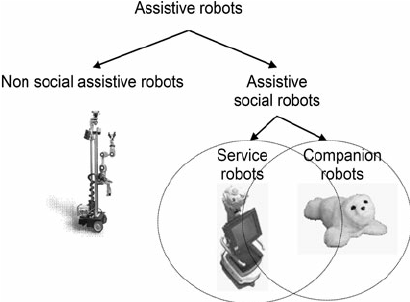
\includegraphics[scale=0.35]{gambar/kategori-sars.png}
  \caption{Pengategorian \emph{assistive robots} (\citet{cit:heerink2010}).}
  \label{fig:kategorisars}
\end{figure}

\emph{Socially assistive robots} (SARs) merupakan adaptasi dari \emph{assistive technology} yang meliputi keseluruhan sistem robotika yang mampu memberikan bantuan kepada pengguna dalam bentuk interaksi sosial \citep{cit:seifer2005}. \citet{cit:heerink2010} mengategorikan riset terhadap SARs menjadi dua kategori berbeda seperti pada Gambar \ref{fig:kategorisars}.
Kategori pertama mencakup \emph{service robots} yang menawarkan bantuan fisik dan kognitif dan melakukan tugas sebagai pelayan, sedangkan kategori kedua mencakup \emph{companion robot} yang merupakan robot berjenis pendamping sebagai sahabat dan media untuk terapi.

Lebih lanjut Rich dan Sidner \citep{cit:rich2009}, menjelaskan SARs mampu memberikan bantuan kepada pengguna dalam berbagai tingkatan seperti:
(a) mendukung kemampuan fungsional dan kognitif pengguna;
(b) menawarkan pengguna kesempatan untuk meningkatkan partisipasi sosial dan kesehatan psikologis;
(c) menyediakan pemantauan jarak jauh dan berkelanjutan atas status kesehatan pengguna;
dan (d) membina pengguna untuk memfasilitasi promosi perilaku sehat dan pencapaian tujuan yang berhubungan dengan kesehatan.

\section{Robot Operating System 2 (ROS 2)}
\label{sec:robotoperatingsystem}

Robot Operating System (ROS) \citep{cit:quigley2009} merupakan kumpulan dari \emph{libraries}, \emph{drivers}, dan \emph{tools} yang mempermudah pengembangan sistem pada robot.
ROS memiliki \emph{command tool} seperti Linux, sistem komunikasi antar proses, dan berbagai macam \emph{packages} yang berhubungan dengan pengembangan sistem pada robot.
Proses yang dieksekusi pada ROS disebut sebagai \emph{node}, komunikasi antar proses yang dimiliki menggunakan model \emph{publish/subscribe}, dan data komunikasi yang dikirimkan disebut sebagai \emph{topic}.

\begin{figure} [ht]
  \centering
	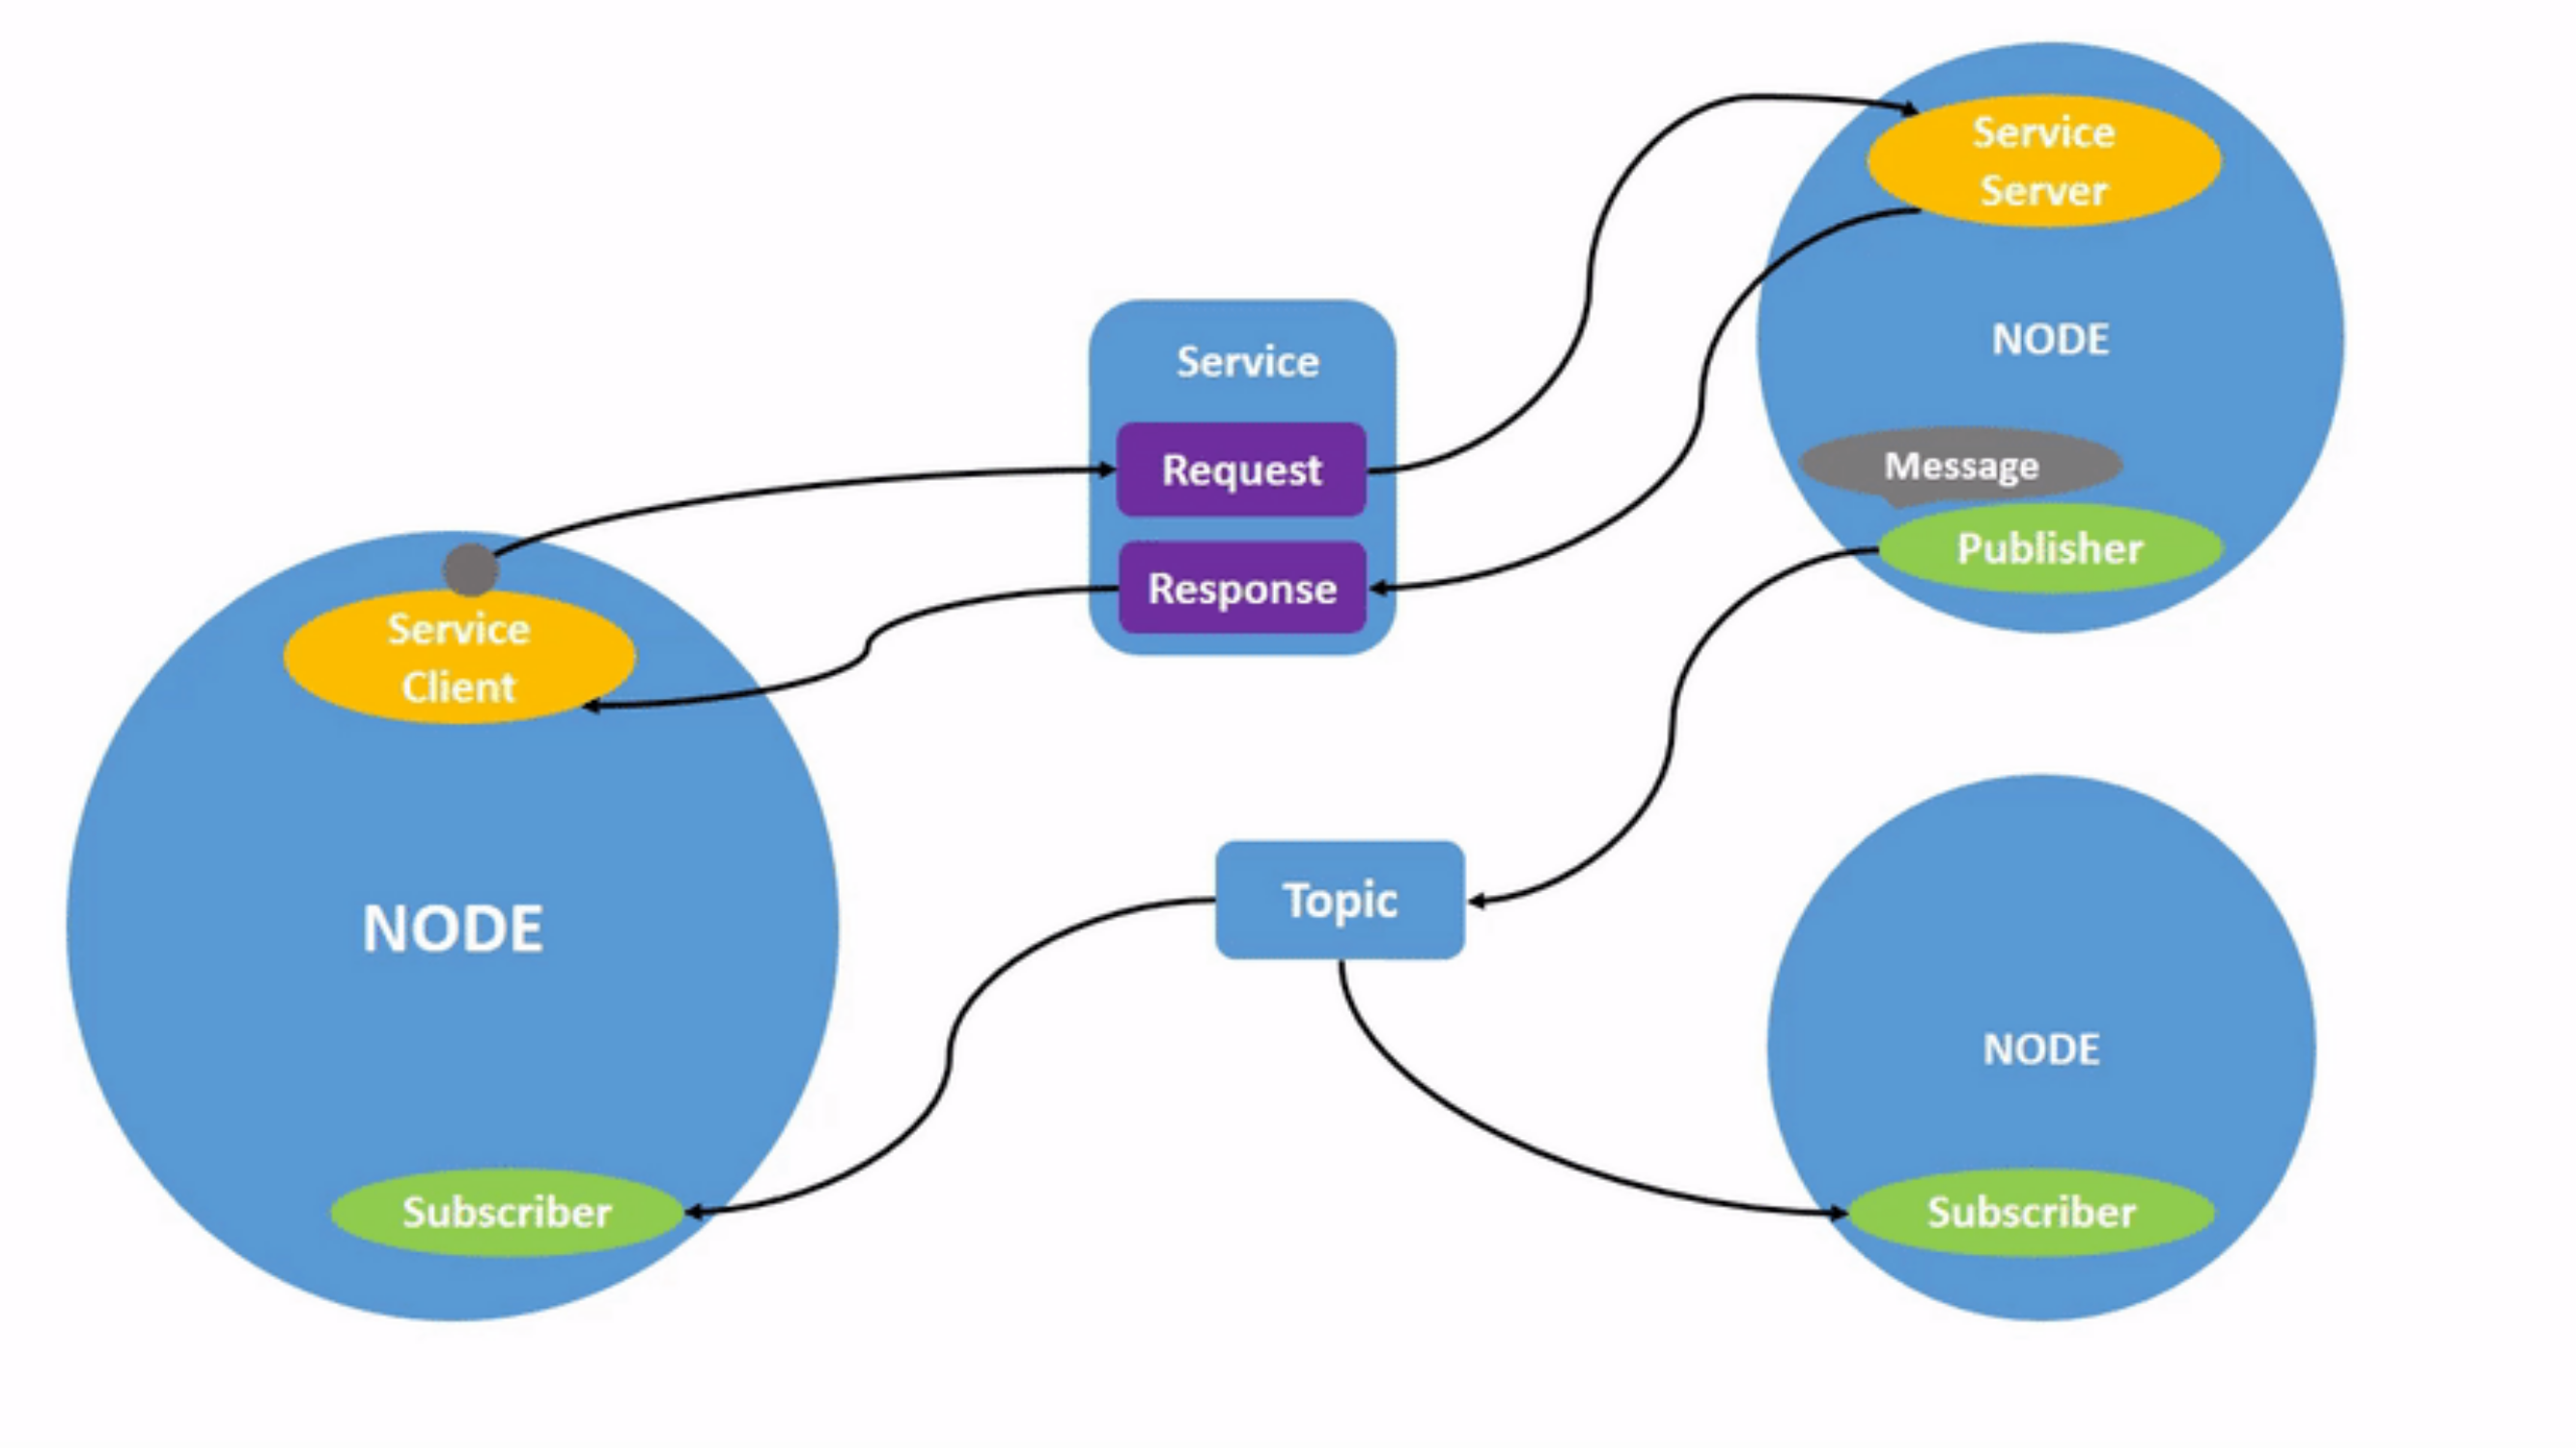
\includegraphics[scale=0.4]{gambar/komunikasi-ros.png}
	\caption{Diagram komunikasi antar node pada ROS 2 \citep{url:ros2nodes}.}
	\label{fig:komunikasiros}
\end{figure}

Seperti yang terlihat pada Gambar \ref{fig:komunikasiros}, Suatu proses \emph{publisher} mampu mengirimkan satu maupun lebih \emph{topic}, kemudian proses-proses lain yang melakukan \emph{subscribe} pada suatu \emph{topic} bisa memperoleh isi dari \emph{topic} tersebut.
Selain itu ada juga \emph{sevice} yang memiliki fungsi seperti \emph{topic}, hanya saja dilakukan secara dua arah.
\emph{Service} ini bekerja menggunakan model \emph{client/server} dimana \emph{service client} akan mengirimkan data permintaan dalam bentuk \emph{request} dan kemudian \emph{service server} akan mengirimkan data balasan dalam bentuk \emph{response}.

Generasi kedua dari Robot Operating System, ROS 2, merupakan kelanjutan dari ROS yang mengusung reliabilitas dan performa untuk penggunaan \emph{real-time} sembari masih mendukung keunggulan yang dimiliki oleh ROS sebelumnya \citep{cit:maruyama2016}.
Untuk memenuhi kebutuhan reliabilitas dan performa untuk penggunaan \emph{real-time} tersebut, ROS 2 menggunakan \emph{Data Distribution Service} (DDS) \citep{cit:castellote2003} \citep{cit:schlesselman2004}, standar industri untuk sistem komunikasi \emph{real-time} dan \emph{end-to-end middleware}, yang menggantikan sistem komunikasi antar proses yang dimiliki ROS sebelumnya.

\section{Gazebo}
\label{sec:gazebo}

Gazebo \citep{cit:koenig2004} merupakan bagian dari Player Project \citep{cit:gerkey2003} yang memungkinkan sebuah simulasi robot dan aplikasi sensor bekerja di lingkungan simulasi \emph{indoor} maupun \emph{outdoor} tiga dimensi.
Gazebo memiliki arsitektur \emph{client/server} dan model \emph{publish/subscribe} untuk sistem komunikasi antar prosesnya.
Setiap objek simulasi di Gazebo dapat diasosiasikan dalam satu maupun lebih kontroler yang akan memproses perintah untuk mengatur dan menentukan keadaan dari suatu objek.
Data yang dihasilkan oleh suatu kontroler akan dikirim ke \emph{shared memory} menggunakan \emph{Gazebo interfaces} (\emph{ifaces}).
Nantinya \emph{ifaces} dari proses-proses lain dapat membaca data tersebut pada \emph{shared memory}, sehingga memungkinkan komunikasi antar proses antara program yang mengontrol robot dan Gazebo, terlepas dari bahasa pemrograman yang digunakan.

% \subimport{3-gazebo}{1-gazebo-model.tex}
% \subimport{3-gazebo}{2-gazebo-plugins.tex}

